\hypertarget{1}{}

\chapter{Introduction}

\rhead{Introduction}
\lhead{Chapter 1}

\vspace{-1.6cm}

% Gray Line
\begingroup
\color{gray}
\par\noindent\rule{\textwidth}{0.4pt}
\endgroup

\noindent{The volume of unstructured textual information currently available widely surpasses the ability of analysis by a researcher, even if restring it to a domain-specific topic. Biomedical literature is the standard method that researchers use to share their findings mainly in the form of articles, patents and other types of written reports \citep{hearst1999untangling}. Thus, scientific articles are the primary source of knowledge for biomedical relations, including human phenotypes and other biomedical entities, such as genes and diseases. A comprehensive source for articles on this topic is the PubMed\footnote{\url{https://www.ncbi.nlm.nih.gov/pubmed/}, visited at 04/06/2020} platform, combining over 30 million citations, as of the date of this proposal, while providing access to their metadata. Processing this amount of information is only feasible using Text Mining techniques.}

Text mining systems usually include Named-Entity Recognition (NER) \citep{notaro2017prediction}, Named-Entity Linking (NEL), and Relation Extraction (RE) tasks. NER consists of recognizing entities mentioned in the text by identifying the offset of its first and last character. NEL consists of mapping the recognized entities to entries in a given knowledge base. RE consists of the identification of a relation between entities mentioned in a given document. Deep learning is widely used to solve problems such as speech recognition, visual object recognition, and object detection. However, deep learning methods that effectively identify and extract relations between biomedical entities in the text are still scarce \citep{li2017neural}. Deep learning is a type of Machine Learning (ML) method that learns data representations using different levels of data abstraction \citep{lecun2015deep}. Systems that perform RE are increasingly more complex, namely the MIMLCNN \citep{jiang2016relation}, and PCNN+Att \citep{lin2016neural}. These systems use Word2Vec \citep{mikolov2013distributed} word embeddings. Word embeddings aim to capture the syntactic and semantic information about the word \citep{kumar2017survey}. Lately, efforts regarding new pre-trained language representation models have been proposed with BERT \citep{vaswani2017attention,devlin2019bert}, and applied to the biomedical domain with BioBERT \citep{lee2020biobert}, achieving promising results.

These pre-trained models can act as information layers for a robust biomedical RE deep learning model that uses not only the training data but also external sources of knowledge like domain-specific ontologies combined with graph attention mechanisms or semantic similarity measures. External sources of knowledge, such as the Gene Ontology (GO) \citep{ashburner2000gene} and the Human Phenotype Ontology (HPO) \citep{robinson2010human}, can provide highly valuable information for the detection of relations between entities in the text \citep{lamurias2019bo}. The GO combines 45 thousand terms, with over 6 million annotations, 1 million gene products, for 4 thousand species, whereas, the HPO contains over 13 thousand terms and over 156 thousand annotations to hereditary diseases. These knowledge-bases provide not only relevant characteristics about the respective entities but also the underlying semantics of the relations they establish. This information is not expressed directly in the training data but could be of interest to reinforce a relation between two entities in the text.

To the best of current knowledge, there is no Deep Learning RE system that includes in their data representations the information encoded in ontologies combined with other type of semantics to identify and extract relations between biomedical entities in articles.

% ------------------------------> OBJECTIVES

\hypertarget{1.2}{\section{Objectives}}

The ultimate goal of this project is to develop a top-performance RE system that combines deep learning state-of-the-art data representations and semantics. The innovation resides in using external sources of knowledge in the form of structured semantics to add extra information not encoded in the training sets. This system will focus on phenotypic abnormalities and the relations they establish with other biomedical entities, such as genes and diseases, taking into account the particulars of these entities. As a second case study, the system will focus on cancer-nutrition interactions regarding our collaboration with the World Health Organization (WHO).

The three main goals to achieve and their main sub-objectives are:

\begin{enumerate}
\item{Robust Deep Learning System}
\begin{enumerate}
\item{Baseline System with Word2Vec (based on the BO-LSTM system \citep{lamurias2019bo})}
\item{System with BERT/ELMo Word Embeddings (or other state-of-the-art models).}
\item{System with Biomedical Word Embeddings}
\end{enumerate}
\item{Semantics as an Add-on for Relation Extraction Systems}
\begin{enumerate}
\item{Add-on Ontologies}
\item{Graph Attention Mechanisms}
\item{Semantic Similarity Measures}
\end{enumerate}
\item{Specific Applications of the System to the Biomedical Domain}
\begin{enumerate}
\item{PGR Improvement}
\item{Cancer-Nutrition Interactions Dataset Creation}
\item{Adaptation for Non-English Languages}
\end{enumerate}
\end{enumerate}

These objectives, in particular the sub-objectives, will be assessed to determine if its use improves the performance of the main system or if another route needs to be taken into consideration. All these objectives are interconnected, as shown in Figure \ref{figure:objectives}.

\begin{figure}[ht]
\captionsetup{font=small}
\centering
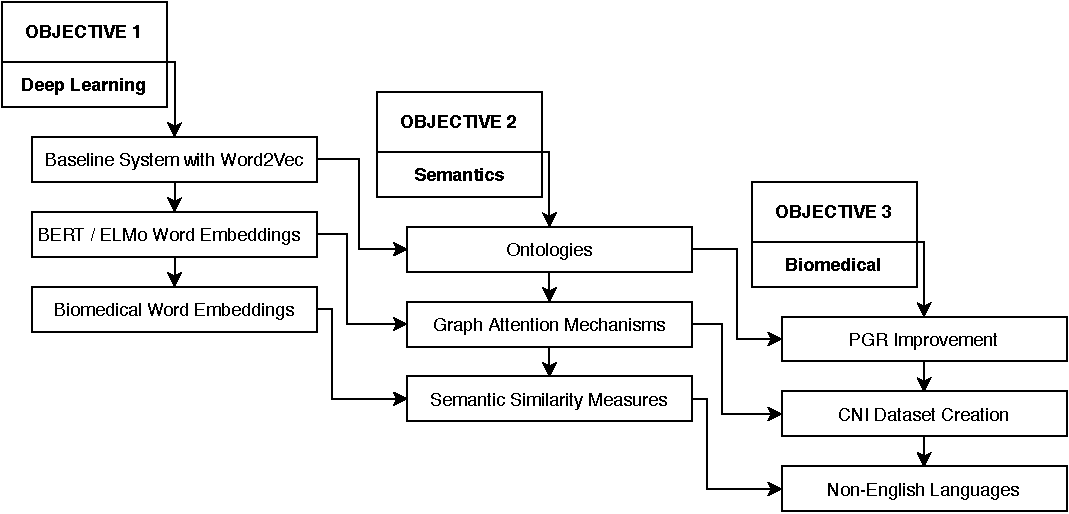
\includegraphics[width=15.5cm]{images/objectives.pdf}
\fontsize{9}{10.8}\caption[Thesis Project Main Objectives]{Main objectives and sub-objectives of the thesis. PGR stands for the Phenotype-Gene Relations dataset and CNI for cancer-nutrition interactions.}
\label{figure:objectives}
\end{figure}

\subsection*{Hypothesis}

\begin{itemize}
    \item Using external sources of knowledge as additional sources of information for deep learning relation extraction systems will improve the number and quality of biomedical relations extracted. These relations can be used to explore new experimental hypotheses providing evidence to researchers and clinicians about possible unknown associations between biomedical entities and populate gold standard knowledge bases.
\end{itemize}


% ------------------------------> METHODOLOGY

%section{Methodology}

%The overall methods to accomplish the proposed objectives can be divided into three stages, one for each objective. The first stage is the creation of a silver standard human phenotype-gene relations corpus (generated in a fully automated manner) (Chapter \hyperlink{3}{3}), the second and third stages are the development of a distantly supervised multi-instance learning module that combines a knowledge base, and the development of a deep learning module that takes advantage of domain-specific ontologies, both for automatic extraction of human phenotype-gene relations (Chapter \hyperlink{4}{4}). 

%To generate a silver standard for phenotype-gene relations, we need a pipeline that performs NER to recognize genes and human phenotype entities, and RE to extract and classify a relation between the identified human phenotype and gene entities. The first step is to gather abstracts using the PubMed API with manually defined keywords, namely, each gene name that participates in a relation (retrieved from a gold standard knowledge base of relations), \textit{homo sapiens}, and \textit{disease}. Then, the NER stage is performed using the Minimal Named-Entity Recognizer (MER) tool \citep{MER} to extract gene mentions, and the Identifying Human Phenotypes (IHP) tool \citep{IHP} to extract human phenotype mentions, from the abstracts. At last, using a gold standard relations knowledge base, provided by the HPO, the relations obtained by co-occurrence of the entities in the same sentence are marked \textit{Known} or \textit{Unknown}, and a subset (test-set) of the relations curated by domain experts. The \textit{Known} relations are in the knowledge base and the \textit{Unknown} relations are not yet identified or that do not exist.
%The test-set was created by randomly selecting 260 relations to be reviewed by eight curators (50 relations each, with an overlap of 20 relations), all researchers working in the areas of Biology and Biochemistry.

%While in the first stage a distant supervision approach is used to mark the relations with \textit{Known} or \textit{Unknown}, in the second stage the unlabeled silver standard corpus is going to be used to apply the distantly supervised multi-instance learning approach. These two distant supervision approaches differ in the way they are applied, as we are going to see in the following chapters.  

%In the second stage, the goal is to use the corpus generated in the first stage unlabeled (annotated only with entity mentions) combined with a knowledge base (provided by the HPO), that provides examples for the relations we wanted to extract, to apply distantly supervised multi-instance learning. The best feature of this machine learning approach is the fact that it does not require the relations annotations, only the human phenotype and gene entities mentions, reducing the amount of manual effort necessary.

%For the last stage, the main goal is to combine RNN (deep learning) algorithms with biological ontologies to improve the identification of human phenotype-gene relations in biomedical literature. Ontologies such as the HPO and the Gene Ontology provide a reliable representation of their respective domains and can be used as data representation layers to extract relations from text. The proposed system is going to represent each candidate pair as the sequence of the relations between the entities ancestors in their respective ontology and combine word embeddings and WordNet (generic English language ontology) to produce a model able to extract the \textit{Known} relations from text.

% ------------------------------> DOCUMENT STRUCTURE

\section{Document Structure}

Additionally to the present introductory chapter, this document is structured in four chapters as follows:

\begin{itemize}
   \item \textbf{Chapter \hyperlink{2}{2}} (Related Work) provides an overview of the key concepts to understand Relation Extraction (RE) according to the three main objectives established previously. It also presents some of the initial approaches for RE, by order of complexity. Furthermore, it describes the different deep learning methods and how they can be combined in systems for RE, and the steeps needed for their evaluation. Additionally, it introduces semantics for RE, based on knowledge bases and graphs (e.g., ontologies) and semantic similarity metrics. Finally, it characterizes the case study dataset and presents potential challenges with the human phenotype-gene RE.
   \item \textbf{Chapter \hyperlink{3}{3}} (Methodology) presents a modular description of the deep learning system for biomedical Relation Ex-traction (RE) combining external sources of knowledge (regarding main objectives 1 and 2). Also, the overall evaluation process and particularities of the biomedical case studies (objective 3). Finally, the last subsection will present the project planning according to a timeline regarding the three main objectives’specificities. 
   \item \textbf{Chapter \hyperlink{4}{4}} (Work in Progress) presents the work already developed and in development following the proposed methodology.
   \item \textbf{Chapter \hyperlink{5}{5}} (Conclusion) discusses the main conclusions of this thesis proposal.
\end{itemize}